\section{Prérequis}
Les prérequis de cette formation sont une bonne maîtrise de {\color{monOrange}HTML \& CSS} et de {\color{monOrange}JavaScript}. Si ce n'est pas le cas, suivez d'abord ces deux formations sur la plateforme.

Une connaissance du langage {\color{monOrange}TypeScript} est un plus, même si nous verrons les fondamentaux nécessaires dans la formation. Vous pouvez suivre en parallèle la formation {\color{monOrange}TypeScript} pour approfondir.

Nous recommandons également de faire la formation {\color{monOrange}Git}, au moins les premiers chapitres si vous ne connaissez pas cet outil.

%%%%%%%%%%%%%%%%%%%%%%%%%ù

\section{Introduction à Vue.js}
\subsection{Qu'est ce que Vue.js ?}
{\color{monOrange}Vue.js} est un framework permettant de développer des interfaces utilisateur. Il est développé entièrement en {\color{monOrange}TypeScript} depuis sa version 3.

{\color{monOrange}TypeScript} est un langage de programmation open source développé par {\color{monOrange}Microsoft}. C'est un sur-ensemble syntaxique de {\color{monOrange}JavaScript}. Cela signifie que c'est du {\color{monOrange}JavaScript} amélioré, qui permet notamment un typage fort. Il est ensuite transformé en {\color{monOrange}JavaScript}. Les navigateurs ne comprennent en effet que les langages {\color{monOrange}HTML}, {\color{monOrange}CSS} et {\color{monOrange}JavaScript}.
\\

Vue.js est fondé sur deux concepts clés : le rendu déclaratif et la réactivité.
\begin{itemize}
\item Le rendu déclaratif est le fait de décrire le rendu ({\color{monOrange}HTML}) en fonction de l'état de l'application (en {\color{monOrange}JavaScript}).
\item La réactivité est le fait que Vue suit les changements d'état dans le code {\color{monOrange}JavaScript} et met à jour le {\color{monOrange}DOM} de manière optimisée si des changements doivent être faits.
\end{itemize}


\subsection{Un framework progressif}
L'une des grandes forces de {\color{monOrange}Vue.js} est d'être progressif : vous pouvez faire une application très simple sans étape de {\color{monOrange}build} juste avec la librairie {\color{monOrange}core}, mais vous pouvez aussi faire une application très complexe avec beaucoup d'étapes de {\color{monOrange}build} automatisés, une gestion des routes, de l'état de l'application etc.

Nous verrons ainsi notamment les librairies officielles suivantes, qui font partie du framework {\color{monOrange}Vue.js} :
\begin{enumerate}
\item {\color{monOrange}Vue Router} : permet de gérer la navigation de l'utilisateur dans l'application.
\item {\color{monOrange}Pinia} : permet de gérer l'état de l'application.
\item {\color{monOrange}Vite} : permet de construire l'application (par exemple en transpilant le {\color{monOrange}Sass} et {\color{monOrange}CSS} ou le {\color{monOrange}TypeScript} en {\color{monOrange}JavaScript}) et de l'optimiser.
\item {\color{monOrange}Transpiler} signifie convertir dans un autre langage de même niveau (contrairement à la compilation qui transforme du code dans un langage de haut niveau à un langage plus proche du langage machine).
\end{enumerate}
\subsection{Tous les rendus possibles !}
{\color{monOrange}Vue.js} permet aujourd'hui de faire des applications de tous les principaux types de rendu :
\begin{itemize}
\item {\color{monOrange}SPA} (Single-Page Application) : le serveur envoie une page {\color{monOrange}HTML} avec un lien vers des fichiers {\color{monOrange}JavaScript} qui contiennent toute l'application. Le navigateur va charger toute l'application qui va gérer un grand nombre d'opérations comme le routage entre les pages.

\item {\color{monOrange}SSR} (Server Side Rendering) : la page {\color{monOrange}Web} est générée par le serveur qui construit le {\color{monOrange}HTML}, le {\color{monOrange}CSS} et le {\color{monOrange}JavaScript} nécessaires en fonction de la requête, pour rendre la page. Pendant ce temps, le navigateur télécharge la {\color{monOrange}SPA} qui sera ensuite utilisée. Cela permet aux utilisateurs d'avoir un premier affichage quasi-immédiat sans avoir à attendre le chargement de l'application. Lorsque le {\color{monOrange}SSR} est configurée on dit alors que l'application est universelle car elle est rendue à la fois côté serveur et côté client. Nous reviendrons en détail sur ces notions dans la formation.

\item {\color{monOrange}SSG} (Static-Site-Generation / JAMStack ) : toutes les pages sont pré-générées sur le serveur (tout le {\color{monOrange}HTML}, le {\color{monOrange}CSS} et le {\color{monOrange}JavaScript} est générés en amont) et servies au navigateur en fonction des requêtes. C'est utile pour faire de petits sites statiques. Vous pouvez alors utiliser {\color{monOrange}VitePress}, la librairie {\color{monOrange}SSG} officielle de {\color{monOrange}Vue}.

\end{itemize}
Vous pouvez également faire des applications bureautiques (par exemple avec {\color{monOrange}Electron} ou {\color{monOrange}Tauri}), des applications mobiles (par exemple avec {\color{monOrange}Ionic} ou {\color{monOrange}Quasar}) ou encore utiliser {\color{monOrange}WebGL} ou développer des applications pour le terminal.

\subsection{Une traction incroyable}
Contrairement à {\color{monOrange}Angular} ou {\color{monOrange}React} aucun géant du numérique ne se cache derrière {\color{monOrange}Vue.js} mais seulement {\color{monOrange}Evan You}, et bien sûr de très nombreux contributeurs. {\color{monOrange}Vue.js} a une traction phénoménale ces dernières années : il dépasse les 3 millions de téléchargements par semaine sur {\color{monOrange}npm} ! C'est le framework {\color{monOrange}JavaScript} qui a le plus d'étoiles sur {\color{monOrange}Github} (environ 200 000).

Le framework est aujourd'hui très stable et est utilisé notamment par {\color{monOrange}Laravel} (comme framework {\color{monOrange}Javascript} par défaut), par {\color{monOrange}GitLab} et par {\color{monOrange}PageKit}. En Chine, il s'agit du framework le plus utilisé avec notamment {\color{monOrange}Alibaba}, {\color{monOrange}Baidu}, {\color{monOrange}Sina Weibo} et {\color{monOrange}Xiaomi} qui l'utilisent en production.

Nous pouvons donner quelques autres exemples de sites connus faits avec {\color{monOrange}Vue.js} : {\color{monOrange}Gitlab, Behance, Upwork, Back Market, Louis Vuitton USA, Ecosia, Google Carreers}, plusieurs sites de {\color{monOrange}Microsoft} (par exemple {\color{monOrange}Azure for Partners}), de très nombreux sites d'{\color{monOrange}Alibaba, Baidu},

\subsection{Vue.js 3}
{\color{monOrange}Vue.js 3} est sorti en septembre 2020 et est devenu la version officielle par défaut en février 2022 (le temps que les autres librairies du framework soient également réécrites). L'ensemble du framework a été entièrement réécrit en {\color{monOrange}TypeScript} et a de bien meilleures performances que la version 2. Il est encore plus léger et optimisé. Il bénéficie également d'une toute nouvelle API appelée {\color{monOrange}Composition API} qui permet de rendre plus facile le développement d'applications complexes.

{\color{monOrange}Vue.js 3} est donc une nouvelle version vraiment différente de la version 2 avec de nombreuses modifications. Les librairies composants le framework ont également changé : {\color{monOrange}Vite} a remplacé {\color{monOrange}Webpack} et {\color{monOrange}Pinia} a remplacé {\color{monOrange}Vuex} par exemple.

\subsection{Avantages}
\begin{description}
\item[Taille]
La librairie {\color{monOrange}Vue.js} fait seulement {\color{monOrange}20kB} lorsqu'elle est minimisée et compressée, c'est donc un {\color{monOrange}framework} très léger qui se charge instantanément par le client.

\item[Rapidité]
Les performances de {\color{monOrange}Vue} sont excellentes et elles surpassent même celles de React sur le rendu et la mise à jour du {\color{monOrange}DOM. Vue.js} utilise un {\color{monOrange}DOM} virtuel pour minimiser le nombre de mutations du {\color{monOrange}DOM} nécessaires lors de changements. {\color{monOrange}Vue.js} a des algorithmes de calcul des mutations nécessaires qui s'avèrent plus performants et légers que ceux de {\color{monOrange}React}.

\item[Un framework complet]
{\color{monOrange}Vue} comporte tous les éléments pour une application moderne complexe : gestion de la navigation, gestion avancée de l'état, gestion de la construction de l'application de manière optimisée, gestion des rendus (même universel avec le {\color{monOrange}SSR}) etc. Autrement dit, {\color{monOrange}Vue} gère tout !
\end{description}
\subsection{Note sur le choix des technologies}
Dans cette formation, nous suivrons l'intégralité des recommandations officielles de {\color{monOrange}Vue.js} et/ou d'{\color{monOrange}Evan You} pour le choix des technologies. Pour cette raison, nous utiliserons {\color{monOrange}TypeScript, Vite}, le {\color{monOrange}Router Vue, Pinia, Visual Studio Code, Volar, Vue browser devtools, Cypress, Vitest, eslint-plugin-vue} et {\color{monOrange}Jest}.

Il est possible de ne pas utiliser ces technologies, ou d'en utiliser d'autres mais nous le déconseillons très fortement car ce serait sortir du maintien et de l'évolution souhaitées par les équipes de Vue.js.

%%%%%%%%%%%%%%%%%%%%%%%%%%%%%%%%%%%%%%%%%%%%%%%%%%%%%%%%%

\section{SPA, create-vue et Vite}
\subsection{Les Single Page Applications}
Comme nous l'avons vu précédemment, {\color{monOrange}Vue.js} permet de construire des {\color{monOrange}Single Page Applications}. Vous connaissez forcément des {\color{monOrange}SPA : Gmail, Google Analytics, Trello, Dropbox} en sont des exemples parmi tant d'autres. La plupart des {\color{monOrange}frameworks} ont adopté cette architecture ({\color{monOrange}Vue, Angular, React, Ember, Meteor} etc).

Nous allons maintenant un peu plus détailler les {\color{monOrange}SPA}. Une single page application ({\color{monOrange}SPA}) est une application qui fonctionne dans un navigateur sans que l'utilisateur n'ait besoin de recharger la page. Le principe est de simuler une application hors ligne : pas de rechargement des pages, de la rapidité, pas d'attente supplémentaire dûe au réseau etc. Les principales caractéristiques de la SPA sont :
\begin{itemize}
\item le rendu est effectué côté client (quand un élément change, la page est modifié grâce aux scripts de l'application chargée côté client).
\item pour fonctionner elle charge en principe une seule fois l'application ({\color{monOrange}HTML, CSS et JavaScript}).
\item seules les données sont transmises, si nécessaire, entre le serveur et l'application client (le plus souvent au format {\color{monOrange}JSON}).
\item le développement mobile est simplifié car le code backend peut être utilisé que l'application soit Web ou native ({\color{monOrange}iOS, Android}).
\item elle est particulièrement adaptée pour stocker les données localement et n'envoyer des requêtes au serveur que lorsque c'est nécessaire.
\end{itemize}

\subsection{La librairie create-vue}
{\color{monOrange}create-vue} est la librairie officielle de {\color{monOrange}Vue.js} permettant de construire facilement un projet avec {\color{monOrange}Vue.js}. Elle permet de configurer entièrement le framework suivant ses souhaits : utiliser ou non {\color{monOrange}TypeScript}, utiliser ou non {\color{monOrange} JSX} (le langage de template de {\color{monOrange}Reac}), utiliser le Router de {\color{monOrange}Vue}, le gestionnaire d'état, la librairie de tests end-to-end etc. Nous verrons bien sûr à plusieurs reprises comment configurer parfaitement un projet {\color{monOrange}Vue.js} en utilisant la librairie.

\subsection{Fonctionnement de Vite}
\begin{center}

\includegraphics[width=3cm]{images/image01.png}
\end{center}

{\color{monOrange}Vite} est un outil de {\color{monOrange}build} conçu par le créateur de {\color{monOrange}Vue.js} pour remplacer {\color{monOrange}Webpack}. C'est donc tout naturellement que {\color{monOrange}Vue.js} recommande aujourd'hui cet outil de {\color{monOrange}build} pour réaliser des applications.

{\color{monOrange}Vite} vient du français, comme {\color{monOrange}Vue, Evan} devant être un amateur de la langue de Molière. Les deux principales fonctionnalités de {\color{monOrange}Vite} sont un serveur de développement et un outil de {\color{monOrange}build} pour la mise en production. {\em Le serveur de développement }: permet d'accéder à l'application durant le développement et de recharger ou de réafficher l'application lors de modifications du code de la manière la plus rapide possible.

\subsubsection{La notion de {\color{monOrange}bundler} ("empaqueteur")}
\begin{center}
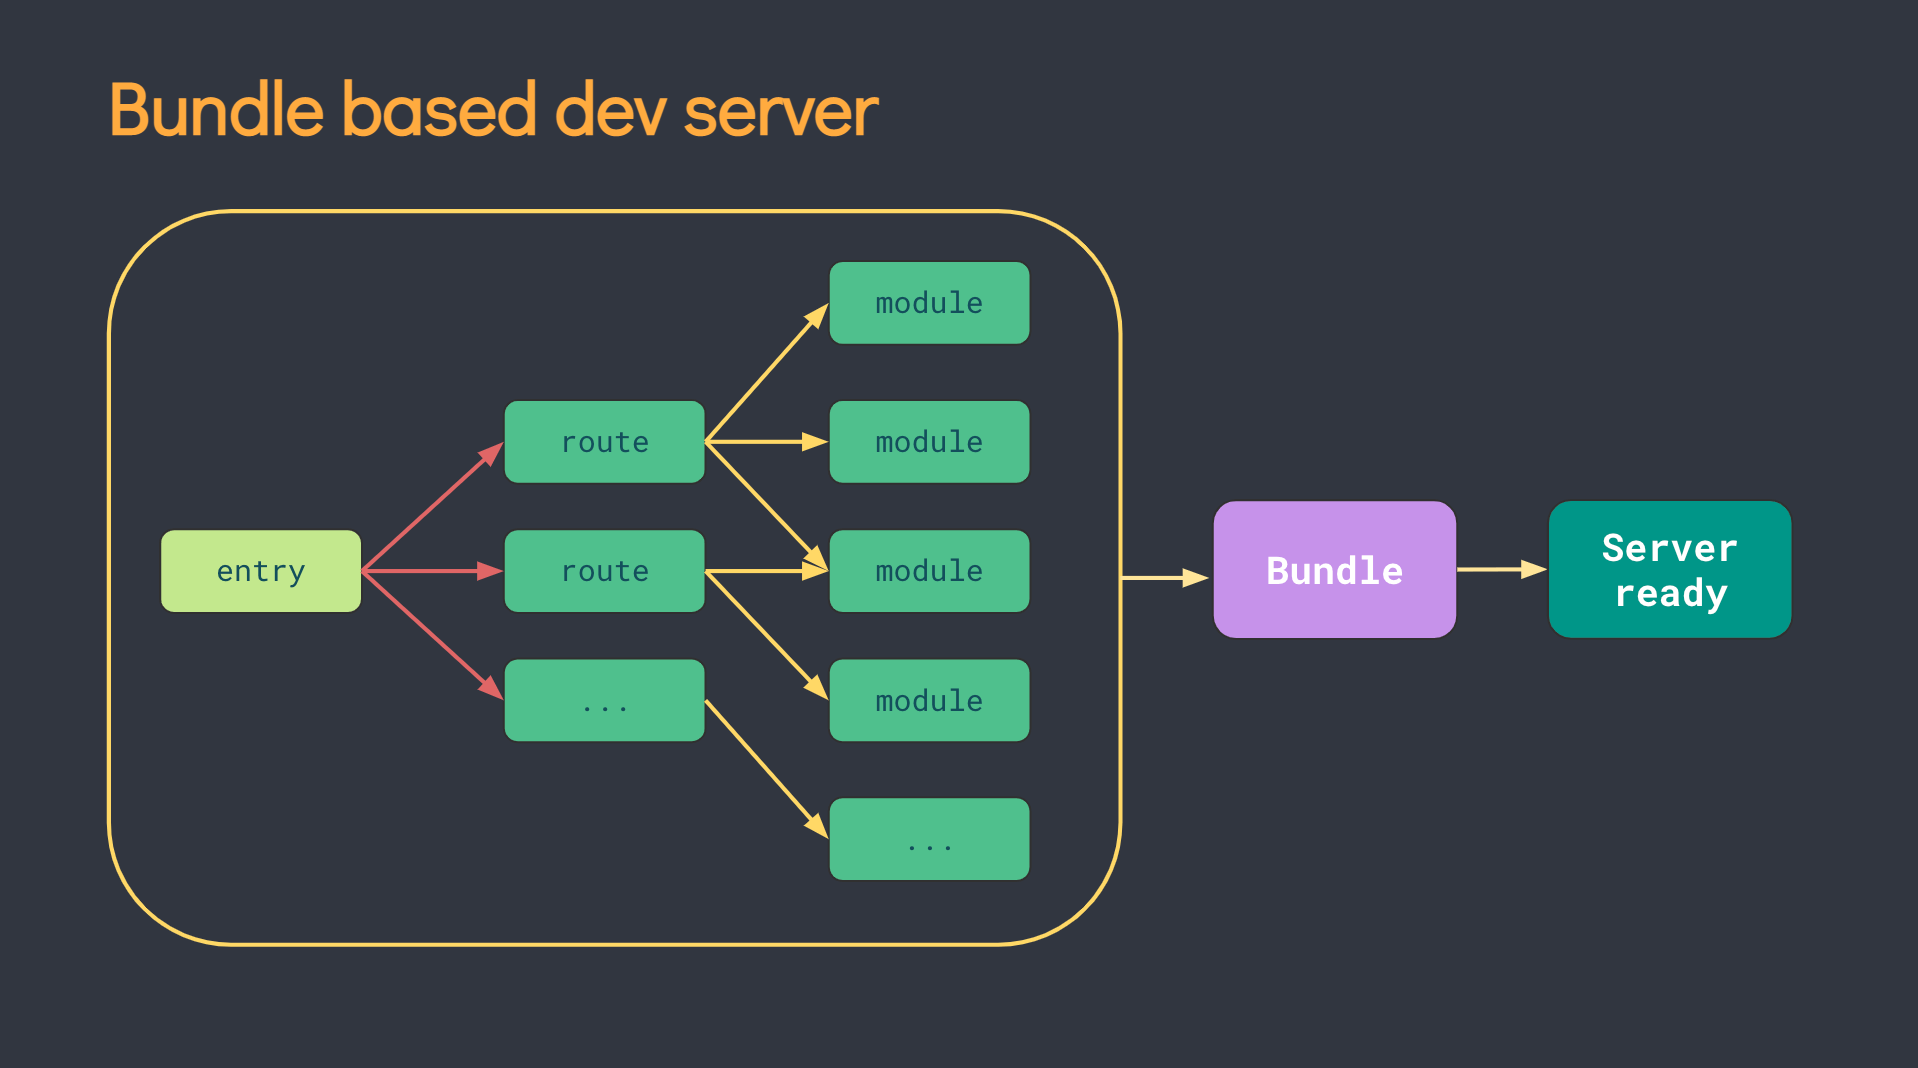
\includegraphics[width=10cm]{images/image02.png}
\end{center}
Un {\color{monOrange}bundle} est un regroupement des fichiers {\color{monOrange}JavaScript, HTML} et {\color{monOrange}CSS} permettant d'accélérer le chargement.

Aujourd'hui, les applications web sont devenues très sophistiquées, c'est pourquoi les frameworks comme {\color{monOrange}Vue.js} morcellent le {\color{monOrange}JavaScript}, le {\color{monOrange}CSS} et le {\color{monOrange}HTML} en de nombreux fichiers afin que le code soit maintenable et réutilisable. Il n'est ainsi pas rare qu'une application complexe dépasse le millier de fichiers.

Les {\color{monOrange}frameworks} utilisent des modules {\color{monOrange}JavaScript} et gèrent les dépendances de chaque fichier avec import et export. Les fichiers importent les dépendances dont ils ont besoin parmi celles exportées par d'autres fichiers. Or, les navigateurs {\color{monOrange}Web} ont besoin que les fichiers soient organisés d'une certaine manière pour fonctionner. Un {\color{monOrange}bundler} permet de les organiser de manière optimisée pour les navigateurs.

Un {\color{monOrange}bundler} peut gérer l'arbre de dépendances créés par les imports et exports pour générer des fichiers uniques. Il réalise également d'autres tâches comme la minification et la compression qui permettent d'obtenir des performances bien supérieures (en rendant le code extrêmement compact et parfois même en le compressant).

\subsubsection{Vite en détail}
Pour le développement, {\color{monOrange}Vite} utilise un {\color{monOrange}pré-bundler} pour les dépendances. Il permet de {\color{monOrange}bundler} les dépendances de 10 à 100 fois plus vite que les outils existants car il est écrit dans un langage plus performant pour ce genre de tâche ({\color{monOrange}Go}).

Il utilise également le remplacement à chaud de module ({\color{monOrange}Hot Module Replacement}), la mise en cache des dépendances par le navigateur, le rechargement uniquement des modules modifiés et la mise en cache des ressources non modifiées pour accélérer au maximum les rechargements lors des modifications du code en tirant profit des dernières évolutions des navigateurs et du langage {\color{monOrange}JavaScript} (principalement les modules {\color{monOrange}EcmaScript}, appelés {\color{monOrange}ESM}).

Pour la production, {\color{monOrange}Vite} va regrouper tous les fichiers {\color{monOrange}JavaScript, HTML} et {\color{monOrange}CSS} dans un {\color{monOrange}bundle} découpé en morceaux (appelés {\color{monOrange}chunks}). La taille des {\color{monOrange}chunks} est optimisée pour le chargement par les navigateurs (notamment en tirant profit du nouveau protocole {\color{monOrange}HTTP2}) en évitant les allers-retours (requête client/réponse serveur) au maximum. Les {\color{monOrange}chunks} sont également optimisées pour la mise en cache (seules les parties de l'application qui sont modifiées entre deux mises en production auront besoin d'être rechargées par le navigateur). Elles permettent enfin d'être chargées au bon moment suivant la route pour limiter les chargements inutiles de code côté navigateur (c'est ce qu'on appelle le {\color{monOrange}lazy-loading}, nous y reviendrons). Enfin, {\color{monOrange}Vite} permet de {\color{monOrange}tree-shaker} l'application : à savoir enlever automatiquement du {\color{monOrange}bundle} final, toutes les parties de l'application et les dépendances qui ne sont pas utilisées effectivement par l'application.

Pour le développement et la production, {\color{monOrange}Vite} s'assure du pré-traitement ({\color{monOrange}pre-processing}) nécessaire pour que l'application puisse être exécutée par les navigateurs. A titre d'exemple, il va transpiler le {\color{monOrange}TypeScript} en {\color{monOrange}JavaScript} ou le {\color{monOrange}Sass} en {\color{monOrange}CSS}.

{\color{monOrange}Vite} est donc un outil très puissant qui réalise énormément d'opérations qui sont cachées au développeur pour optimiser la productivité lors de la phase de développement et la performance lors de la production de l'application. Une fois qu'on a goûté à {\color{monOrange}Vite}, il n'est plus possible de s'en passer !

\subsubsection{Qu'est-ce que {\color{monOrange}TypeScript} ?}
\begin{center}

\includegraphics[width=2cm]{images/image03.png}
\end{center}

Les projets utilisant {\color{monOrange}JavaScript} se sont complexifiés énormément et il est devenu de plus en plus difficile de les maintenir. Il est compliqué de pouvoir comprendre ce que fait du code {\color{monOrange}JavaScript} lorsqu'on arrive sur un projet impliquant de nombreux développeurs. Il est difficile de savoir ce qu'accepte une fonction et ce qu'elle retourne, et devoir à chaque fois lire les éventuels commentaires pour chaque fonction dans plusieurs fichiers est fastidieux. De très nombreux langages ou environnement ont tenté d'y remédier, on peut citer notamment : {\color{monOrange}Flow, Dart, Elm, Reason}, et {\color{monOrange}Closure}. Mais le seul qui a vraiment conquis l'écosystème et s'est imposé dans une quantité astronomique de projets majeurs est {\color{monOrange}TypeScript}.

{\color{monOrange}TypeScript} a été créé par {\color{monOrange}Microsoft} en 2012, il est depuis le départ un projet open-source. C'est un langage avec un typage fort et qui transpile en {\color{monOrange}JavaScript}. Transpiler signifie compiler vers un langage de même niveau. Il est conçu comme une addition pour faire de {\color{monOrange}JavaScript} un langage qui scale en ajoutant des types. Ses avantages immédiats sont :
\begin{enumerate}
\item  Du code beaucoup plus lisible.
\item  Du code beaucoup plus maintenable.
\item  Beaucoup de {\color{monOrange}bugs} en moins grâce au compilateur.
\end{enumerate}
Depuis la version 3 de {\color{monOrange}Vue.js}, le framework entier est codé en {\color{monOrange}TypeScript} et l'équipe recommande fortement l'utilisation de {\color{monOrange}TypeScript}. Si l'utilisation de {\color{monOrange}TypeScript} peut paraître fastidieuse au départ c'est un investissement extrêmement lucratif ! Les gains de productivité sont énormes. Dans la formation nous utiliserons donc {\color{monOrange}TypeScript} en vous présentant toutes les bases du langage nécessaires. Si vous voulez ensuite aller plus loin, vous pourrez simplement suivre la formation {\color{monOrange}TypeScript} sur la plateforme.

%%%%%%%%%%%%%%%%%%%%%%%%%%%%%%%%%%%%%%%%%%%%%%%%%%%%%%%%%%%%%%%

\section{Environnement GNU/Linux}
\subsection{Installation de {\color{monOrange}Node.js} avec {\color{monOrange}node version manager}}
{\color{monOrange}nvm} permet d'installer et d'utiliser plusieurs versions de {\color{monOrange}Node.js} localement. C'est intéressant si vous avez plusieurs projets à des versions différentes. Installez {\color{monOrange}nvm} :

\begin{minted}[
mathescape,
framesep=2mm,
baselinestretch=1.2,
%fontsize=\small,
bgcolor=LightGray,
%linenos
]{bash}
wget -qO- https://raw.githubusercontent.com/nvm-sh/nvm/v0.39.1/install.sh | bash
\end{minted}

Collez les commandes suivantes :

\begin{minted}[
mathescape,
framesep=2mm,
baselinestretch=1.2,
%fontsize=\small,
bgcolor=LightGray,
%linenos
]{bash}
export NVM_DIR="$([ -z "${XDG_CONFIG_HOME-}" ] && printf %s "${HOME}/.nvm" || 
printf %s "${XDG_CONFIG_HOME}/nvm")"
[ -s "$NVM_DIR/nvm.sh" ] && . "$NVM_DIR/nvm.sh" # This loads nvm
\end{minted}

Installez {\color{monOrange}Node.js} LTS :

\begin{minted}[
mathescape,
framesep=2mm,
baselinestretch=1.2,
%fontsize=\footnotesize,
bgcolor=LightGray,
%linenos
]{bash}
nvm install --lts
\end{minted}

\subsection{Installation de {\color{monOrange}Node} sans {\color{monOrange}nvm}}
Ouvrez un terminal et entrez la commande suivante qui va installer la version LTS de {\color{monOrange}Node.js} :
\begin{minted}[
mathescape,
framesep=2mm,
baselinestretch=1.2,
%fontsize=\footnotesize,
bgcolor=LightGray,
%linenos
]{bash}
curl -fsSL https://deb.nodesource.com/setup_lts.x | sudo -E bash -
sudo apt-get install -y nodejs
\end{minted}

Vérifiez l'installation :
\begin{minted}[
mathescape,
framesep=2mm,
baselinestretch=1.2,
fontsize=\footnotesize,
bgcolor=LightGray,
%linenos
]{bash}
node -v
\end{minted}

\subsection{Installation de {\color{monOrange}VS Code} avec snap sur Ubuntu}
Pour installer l'éditeur {\color{monOrange}VS Code} sur {\color{monOrange}Ubuntu}, nous vous recommandons d'utiliser {\color{monOrange}snap}. Ouvrez un terminal et faites simplement :
\begin{minted}[
mathescape,
framesep=2mm,
baselinestretch=1.2,
%fontsize=\footnotesize,
bgcolor=LightGray,
%linenos
]{bash}
snap install code
\end{minted}

\subsection{Installation de VS Code avec l'installeur}
Si vous êtes sur une autre distribution ou que vous ne souhaitez pas utiliser {\color{monOrange}snap}, vous pouvez également utiliser l'installeur. Il vous suffit de le télécharger ici.

\subsection{Ouvrir un terminal dans {\color{monOrange}VS Code}}
Pour ouvrir la vue "Terminal" sur VS Code vous pouvez au choix :

Utiliser {\color{monOrange}Ctrl+`}. Si le raccourci ne fonctionne pas. Allez dans le menu {\tt File > Preferences > Keymaps}. Ensuite recherchez view toggle terminal. Et choisissez un raccourci puis faites Entrée. Nous recommandons Ctrl et la touche la plus à gauche juste sous la touche d'échappement.
\begin{itemize}
\item Aller dans le menu {\tt View > Terminal}.

\item Aller dans le menu {\tt Terminal > new terminal}.

\item Tapez {\tt Ctrl+Shift+P} puis tapez Toggle terminal puis entrée.
\item Installation d'extensions {\color{monOrange}VS Code}: Allez dans l'onglet extension sur {\color{monOrange}VS Code}. Recherchez et installez {\color{monOrange}Volar, TypeScript Vue Plugin (Volar)} et {\color{monOrange}Material Icon Theme}.
\end{itemize}



%%%%%%%%%%%%%%%%%%%%%%%%%%%%%%%%%%%%%%%%%%%%%%

\section{Environnement macOS}
\subsection{Installation de {\color{monOrange}Node.js}}
Dans le cours vous aurez besoin d'installer des dépendances {\color{monOrange}JavaScript}, appelées {\color{monOrange}packages}, nous vous conseillons donc d'installer {\color{monOrange}npm} qui est le gestionnaire de dépendances de {\color{monOrange}Node.js}.
\begin{itemize}
\item Si vous n'avez pas npm, installez Node.js (qui comprend npm) : ici en sélectionnant l'installeur MacOS.
\item Si vous préférez utiliser homebrew, ouvrez un terminal et faitres :
\begin{minted}[
mathescape,
framesep=2mm,
baselinestretch=1.2,
%fontsize=\footnotesize,
bgcolor=LightGray,
%linenos
]{bash}
brew install node
\end{minted}

\end{itemize}
\subsection{Installation de VS Code}
Pour installer l'éditeur {\color{monOrange}VS Code}, avec l'installeur télécharger le ici.

\subsection{Ouvrir un terminal dans {\color{monOrange}VS Code}}
Pour ouvrir la vue "Terminal" sur VS Code vous pouvez au choix :

Utiliser {\color{monOrange}Ctrl+`}. Si le raccourci ne fonctionne pas. Allez dans le menu {\tt File > Preferences > Keymaps}. Ensuite recherchez view toggle terminal. Et choisissez un raccourci puis faites Entrée. Nous recommandons Ctrl et la touche la plus à gauche juste sous la touche d'échappement.
\begin{itemize}
\item Aller dans le menu {\tt View > Terminal}.

\item Aller dans le menu {\tt Terminal > new terminal}.

\item Tapez {\tt Ctrl+Shift+P} puis tapez Toggle terminal puis entrée.
\item Installation d'extensions {\color{monOrange}VS Code}: Allez dans l'onglet extension sur {\color{monOrange}VS Code}. Recherchez et installez {\color{monOrange}Volar, TypeScript Vue Plugin (Volar)} et {\color{monOrange}Material Icon Theme}.
\end{itemize}




